\documentclass{article}
\usepackage[UTF8]{ctex}
\usepackage{geometry}
\usepackage{multirow}
\usepackage{natbib}
\geometry{left=3.18cm,right=3.18cm,top=2.54cm,bottom=2.54cm}
\usepackage{graphicx}
\pagestyle{plain}	
\usepackage{setspace}
\usepackage{enumerate}
\usepackage{caption2}
\usepackage{datetime} %日期
\renewcommand{\today}{\number\year 年 \number\month 月 \number\day 日}
\renewcommand{\captionlabelfont}{\small}
\renewcommand{\captionfont}{\small}
\begin{document}

\begin{figure}
    \centering
    
\includegraphics[width=8cm]{upc.png}

    \label{figupc}
\end{figure}

	\begin{center}
		\quad \\
		\quad \\
		\heiti \fontsize{45}{17} \quad \quad \quad 
		\vskip 1.5cm
		\heiti \zihao{2} 《计算科学导论》个人职业规划
	\end{center}
	\vskip 2.0cm
		
	\begin{quotation}
% 	\begin{center}
		\doublespacing
		
        \zihao{4}\par\setlength\parindent{7em}
		\quad 

		学生姓名:\underline{\qquad  王烁 \qquad \qquad}

		学\hspace{0.61cm} 号:\underline{\qquad 1907010212}
		
		专业班级:\underline{\qquad 本研人工智能 \qquad  }
		
        学\hspace{0.61cm} 院:\underline{计算机科学与技术学院}
% 	\end{center}
		\vskip 1.5cm
		\centering
		\begin{table}[h]
            \centering 
            \zihao{4}
            \begin{tabular}{|c|c|c|c|c|c|c|c|c|}
            % 这里的rl 与表格对应可以看到,姓名是r,右对齐的;学号是l,左对齐的;若想居中,使用c关键字。
                \hline
                \multicolumn{5}{|c|}{分项评价} &\multicolumn{2}{c|}{整体评价}  & 总    分 & 评 阅 教 师\\
                \hline
                自我 & 环境 & 职业 & 实施 & 评估与 & 完整性 & 可行性 &\multirow{2}*{} &\multirow{2}*{}\\
                分析& 分析& 定位 & 方案 & 调整 & 20\% & 20\% & ~&~ \\\            
                10\% & 10\% & 15\% & 15\% & 10\% & &  &~ &~\\
                \cline{1-7} 
                & & & & & & & ~&~ \\
                & & & & & & & ~&~ \\
                \hline      
            \end{tabular}
        \end{table}
		\vskip 2cm
		\today
	\end{quotation}

\thispagestyle{empty}
\newpage
\setcounter{page}{1}
% 在这之前是封面,在这之后是正文
\section{自我分析}
	尼采曾经说过 “人生中最难的阶段不是没人懂你,而是你不懂你自己”。作为大一新生,面对未来可能从事的各样职业,我们不禁感到迷茫与困惑,究竟什么才是最适合自己的呢?我们又该选择怎样的人生道路呢?那么首先,我们必须了解自己。\par
	自我分析包括:\par
\subsection{自然条件}
我叫王烁,是一个来自安徽六安的18岁男孩,热爱运动,身体健康,体魄强健,现就读于山东省青岛市中国石油大学(华东)。\par
\subsection{性格分析}
从小时候我就是个坐不住板凳的人,特别爱这折腾,总是喜欢到处乱跑也很调皮烦人,是个典型的外向热情的男孩子。但随着年龄的增长,可能是因为吃过的亏多了,遭遇的尴尬多了,也可能是因为我明白了原来不知道的道理,我开始变得更加 “冷静”,我会开始理性地思考问题,不在一味地躁动烦人,但同时我也更加“胆怯”,我自己能清晰地发现现在的我会主动拒绝对我而言更多的表现机会与挑战。尤其是经历了高中绝望的生活后,所有的一切都被压抑进书本里,我变得理性,清醒,也变得缺乏勇气和没有自信。但“冷漠”只是我后天形成的外表,其内在仍然是那个活泼暴躁的小破孩,我还是渴望表现自我,展现自己的能力。在大学的生活里,多了许多生活与交际的问题,而我也变得更加矛盾,每当我面临选择之时,我总是犹豫不知所措,或三思咬牙一试,或沉默放弃。\par
\subsection{教育与学习经历}
我小学是在安徽省六安市三十铺镇一小小学念书,愉快的玩耍6年过后,我开始了3年六安汇文中学的磨砺读书征程,之后去了六安第一中学,又经历了3年盼天盼地的学习,我踏入了中国石油大学(华东),开始了又一新的旅程。\par
\subsection{工作与社会阅历}
暂无工作,也没有工作过,现在的主要任务是学习。对社会的认识尚浅,只参加过一些志愿者活动,由于父母的宠爱,也没有经历生活苦难的打磨。虽然还未有太多社会阅历,但我不惧以后的生活,期待未来的挑战。希望将来踏入社会后能适应生活,找到一份薪水满意并且自己喜欢的工作。\par
\subsection{知识、技能与经验}
掌握了数理化生等基本中学知识,对生活中的事物与自然规律有了新的浅薄的认识。经历了中考与高考以及数不清的考试后,已经对于学习有了一套烂熟于心的方法,并且对于如何应对与通过考试有了自我理解,掌握了丰富的应考经验,可以做到无畏考试,接受考试,战胜考试。如今,对于数学分析与线性代数仍处于迷茫时期,开始学习并正在掌握计算机相关的知识,着力培养自己的科学素养,专业方面的知识正在完善。\par
\subsection{兴趣爱好与特长}
喜欢运动,热衷于长跑,曾在学校5000m长跑比赛中取得优异成绩。喜欢听音乐,会拉二胡,虽然自己五音不全,但很喜欢沉浸在旋律的舞动中。平时闲暇之余,会与朋友相约篮球场,来场痛快的对决。沉迷阅读小说,尤其是侦探与科幻类型,超级喜欢可以很好的结合它们与情感线灵魂线的作家,比如马克•李维,大刘等。对于少年热血小说也情有独钟。经常观看电影,不喜欢逻辑性不强剧情拖沓细节粗糙的无脑电影,觉得只有在影片结束后能带给人某种思考启迪或者感触共鸣的才是好电影。\par
\section{环境分析}
环境是对人的发展影响最大,未来我们的定位如何,更多的是决定于我们所处的环境。\par
环境分析包括:\par
\subsection{社会环境分析}
当今国际政治格局瞬息万变,世界多极化愈演愈烈,科技革命加速前进,中国与美国的矛盾日益加重。由于中国的信息科学发展很快速,中国的还有许多不完善的地方。中国急需计算机人才,尤其是经过系统培训的高级计算机人才。因此企业计算机职业市场广阔。  要在中国发展企业,必须要适合中国的国情,这就要求管理的科学性与艺术性和环境动态适应相结合。因此,受中国市场吸引进入的大批外资企业都面临着本土化改造的任务。这就为准备去计算机工作的人员提供了很多机会。目前中国市场对IT人才的需求每年超过20万人。\par
\subsection{家庭环境分析}
父母婚姻美满,一起从事个体户经营,经济处于中等小康水平,从小时候起,妈妈和爸爸就希望我好好读书,将来有所出息,所以儿时的我就被严格要求要考个好成绩,直到高中,随着我年龄的增长,爸妈对我学习上的要求也只剩期待了,更多的则是希望我在生活上做个强者,不辜负自己的努力,而学习越来越多变成我自己的事了。上大学前夕,父母对我的要求仅仅是要我保证身体健康,快乐生活。\par
\subsection{职业环境分析}
目前中国市场对IT人才的需求每年超过20万人。IT业一直是国家优先发展的重点行业,也是国内外人才需求量最大的行业之一。伴随着互联网的发展,IT人才的短缺现象将会越来越严重。在我国,IC人才、网络存储人才、电子商务人才、信息安全人才、游戏技术人才严重短缺。未来一段时间社会仍对计算机专业高端人才有很大需求,但计算机专业毕业生也将会面临日趋激烈的竞争。\par
工作内容:计算机专业拥有着广阔的就业前景,因此作为主打专业,该毕业生可从事的专业非常多,主要面向交通系统各单位、各类计算机专业化公司、广告设计制作公司、汽车营销技术服务等从事IT行业工作。\par
工作要求:具有足够的计算机思维、工程能力和数字化、算法、模块化与层次化等核心专业意识,具备满足工程实践需求的计算学科知识体系,能和团队进行合作配合,培养不断探索进取的精神。\par
发展前景:随着科技的进步和信息事业的发展,尤其是计算机技术的发展与网络应用的逐渐普及。计算机已成为人们工作和生活中不可缺少的东西。IT行业迅猛发展,就业工作岗位比比皆是,但是面临的竞争也非常激烈。
\par
\subsection{地域与人际环境分析}
青岛地处北温带季风区域,温度适中,四季分明。属于沿海一线城市,经济实力雄厚,对于IT人才来说有着诸多就业选择。如果将来我没有选择留在青岛,我可能会去南京工作,那里师资力量雄厚,实践机会多,经济较为发达,且属于发展前景较大,机会较多,相对经济压力不会太大的二线城市中的翘首。\par
\par 
\begin{figure}[h!]
\centering
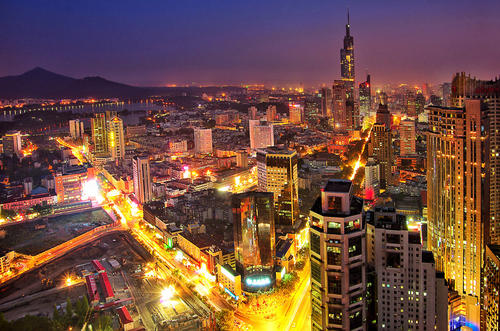
\includegraphics[scale=2.8]{u=3926568172,3413445647&fm=26&gp=0}
\caption{南京}
\label{fig:universe}
\end{figure}



\section{职业定位}
\par
职业定位包括:\par

\subsection{行业领域定位与理由}
基于我是本研一体班的学生,将来极大概率从事人工智能有关的研究,而最近对我们导师带领的师哥师姐的生成对抗网络(GAN)项目感到兴趣,我可能从事软件工程师或有关机器学习领域的工作。\par
\subsection{职业岗位起点定位与理由}
我的职业岗位起点将会选择从普通员工做起,对于个人来说,我需要不断培养工作能力与积累经验,而不是好高骛远,并且在学习过程中,着力加强与团队合作的能力,为以后更好的发展打下基础。\par
\subsection{职业目标与可行性分析}
\par
成果目标、经济目标、能力目标、职务目标等。\par 
\begin{enumerate}[(2)]
	\item 短期目标(大学4年)
\end{enumerate}
\begin{table}[!htbp]   
	\newcommand{\tabincell}[2]{\begin{tabular}{@{}#1@{}}#2\end{tabular}}
	\centering
	\begin{center}  
		\renewcommand{\arraystretch}{2}
		\begin{tabular}{|c|c|c|c|}  
			\hline  
			年级 & 致力方向 & 目的 & 具体目标 \\ \hline  
			大一& \tabincell{c}{C++、英语、数学分析、\\线性代数等基础课程} & \tabincell{c}{打下良好的科学基础,\\培养科学文化素养}& \tabincell{c}{各科成绩达到70分以上\\拿到全国大学生英语四级证书} \\ \hline  
			大二 & \tabincell{c}{基础课程、专业课  \\} &\tabincell{c}{ 继续巩固自己的\\专业基础} & \tabincell{c}{拿到全国大学生英语六级证书 }\\
			\hline  
			大三 & \tabincell{c}{学习专业知识,积极探索导师领导课题\\再次明确自己的方向}&\tabincell{c} {提高专业知识水平\\丰富社会经验} & \tabincell{c}{参加专业竞赛;\\进入到老师的\\实验室参与研究项目} \\ \hline
			大四 & \tabincell{c}{跟随导师做项目,\\实习} & 了解公司运营模式,增加经验& 初步选择自己心仪公司 \\ 
			\hline
		\end{tabular}  
	\end{center}  
\end{table}
\begin{enumerate}[(1)]
	\item 中期目标(大学4年)
\end{enumerate}
\begin{itemize}
    \item 保持优异的成绩在中国石油大学直至研究读完,并积极跟随导师做相关的课题研究,增加实习经验。\par
    \item 进入适合自己发展的公司,开始努力工作并不断培养自己。
\end{itemize}


\section{实施方案}
在明确了职业定位后,要制定实现职业生涯目标的行动方案,不付诸行动,职业目标只能是一种梦想。实施方案是实现职业目标的保证,尽量考虑周全、具有可操作性。\par
实施方案可以从以下角度考虑:\par
\begin{enumerate}[I]
	\item 我会保持阅读量与观影量,增加人文素养,提高自己创造能力与思考能力,积极发展相关知识的兴趣与构造。
	\item 我会克服懒惰,怯场等性格,制定严格规划,主动参加实践活动,锻炼与他人相处合作能力。
	\item 我会真诚待人,利用已有人脉资源,结交更多上进优秀的同伴,扩大人际网络。
	\item 我会主动留下适量时间陪伴家人,若非特殊情况,保证自己能和家人度过周末假日。为家人创造良好环境,营造安全氛围,及时倾听他们的心声。
	\item 烦恼压力大的时候,多去运动,或相约几个知心好友出去狂欢。懂得劳逸结合,保证自己的工作质量与效率。
\end{enumerate}
\par 
\section{评估与调整}
由于影响职业生涯规划的因素很多,且大都处于动态变化之中,因此职业生涯规划应定期评估,并根据影响因素的变化和实施结果的情况及时作出调整,这样才能保证其行之有效。\par 
\subsection{评估时间}
我决定每学年评估一次。\par
\subsection{评估内容}
我将评估自己是否达到自己计划目标,完成相应成果,自己的能力是否已达预期水平,自己的职务与自己的期望是否相符。我会根据现状调整接下来的计划与期望,总结我的收获与缺陷,修改完善我之前的错误问题,保持干劲,继续努力。\par
\subsection{调整原则}
根据我的发展进程,我会确立我是否适合这个职业,或是否仍像刚开始一般抱有极大热情与兴趣。如果我发现更感兴趣的方面,我会及时转型,开展新的发展。\par




\end{document}
